\documentclass{beamer}
\usepackage{tikz}

\usetheme{default}

\title{Ramanujanovi grafi}
\author{Tadej Petrič}

\begin{document}

\begin{frame}[plain]
    \titlepage
\end{frame}

\begin{frame}
    \frametitle{Motivacija}
    Povezave računalniških naprav v omrežju
\end{frame}
\begin{frame}
    \frametitle{Motivacija}
    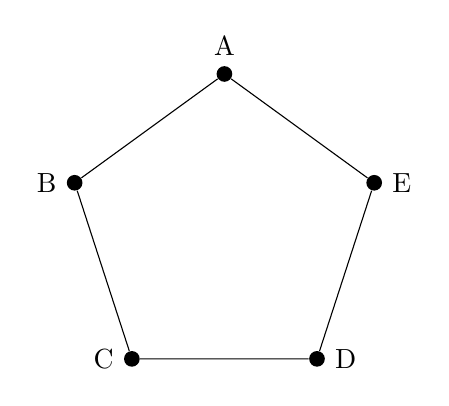
\begin{tikzpicture}
        \node[circle, fill=black, inner sep=2pt, label=above:A] (A) at (90:2) {};
        \node[circle, fill=black, inner sep=2pt, label=left:B] (B) at (162:2) {};
        \node[circle, fill=black, inner sep=2pt, label=left:C] (C) at (234:2) {};
        \node[circle, fill=black, inner sep=2pt, label=right:D] (D) at (306:2) {};
        \node[circle, fill=black, inner sep=2pt, label=right:E] (E) at (18:2) {};
        \draw (A) -- (B) -- (C) -- (D) -- (E) -- (A);
    \end{tikzpicture}
\end{frame}
\begin{frame}
    \frametitle{Motivacija}
    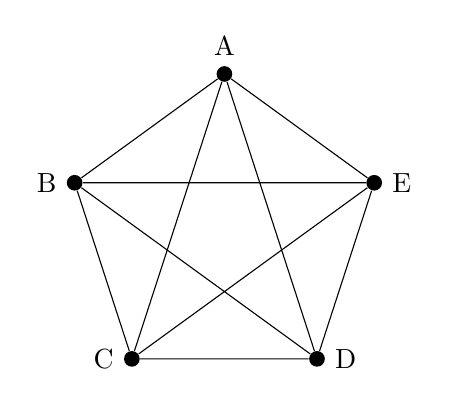
\begin{tikzpicture}
        \node[circle, fill=black, inner sep=2pt, label=above:A] (A) at (90:2) {};
        \node[circle, fill=black, inner sep=2pt, label=left:B] (B) at (162:2) {};
        \node[circle, fill=black, inner sep=2pt, label=left:C] (C) at (234:2) {};
        \node[circle, fill=black, inner sep=2pt, label=right:D] (D) at (306:2) {};
        \node[circle, fill=black, inner sep=2pt, label=right:E] (E) at (18:2) {};
        \draw (A) -- (B) -- (C) -- (D) -- (E) -- (A);
        \draw (A) -- (C) -- (E) -- (B) -- (D) -- (A);
    \end{tikzpicture}
\end{frame}
% BEGIN CHEEGER
\begin{frame}
    \frametitle{Cheegerjeva konstanta}
    Ločevanje grafa na dva dela
    \begin{itemize}
        \item \(G = (V, E)\) povezan graf
        \item \(S \subseteq V\) množica vozlišč (\(|S| \leq \frac{|V|}{2}\))
        \item \(\partial S\subseteq E\) množica povezav od \(S\) do \(\overline S\) \pause
        \item Želimo, da za velik \(|S|\) tudi velik \(\partial S\)
    \end{itemize}
    \pause
    \[
        c(G) = \min_S\frac{|\partial S|}{|S|}
    \]
\end{frame}
\begin{frame}{Primeri - Cheegerjeva konstanta}
    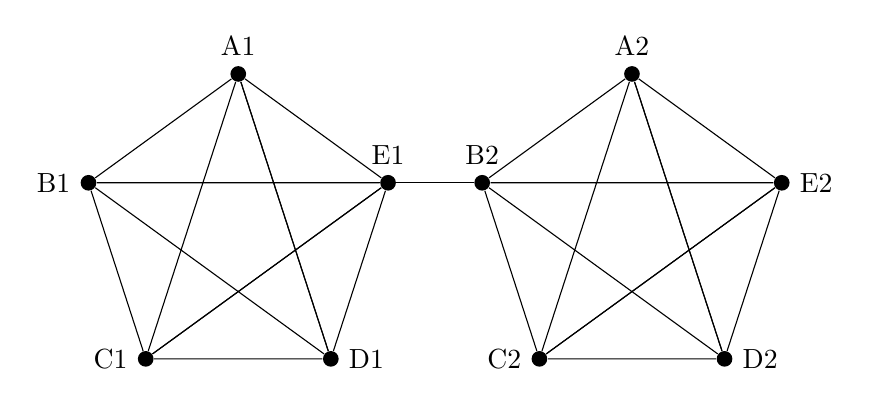
\begin{tikzpicture}
        % First K_5
        \begin{scope}[shift={(0,0)}]
            \node[circle, fill=black, inner sep=2pt, label=above:A1] (A1) at (90:2) {};
            \node[circle, fill=black, inner sep=2pt, label=left:B1] (B1) at (162:2) {};
            \node[circle, fill=black, inner sep=2pt, label=left:C1] (C1) at (234:2) {};
            \node[circle, fill=black, inner sep=2pt, label=right:D1] (D1) at (306:2) {};
            \node[circle, fill=black, inner sep=2pt, label=above:E1] (E1) at (18:2) {};
            \draw (A1) -- (B1) -- (C1) -- (D1) -- (E1) -- (A1);
            \draw (A1) -- (C1) -- (E1) -- (B1) -- (D1) -- (A1);
            \draw (A1) -- (D1);
            \draw (B1) -- (E1);
            \draw (C1) -- (E1);
        \end{scope}

        % Second K_5
        \begin{scope}[shift={(5,0)}]
            \node[circle, fill=black, inner sep=2pt, label=above:A2] (A2) at (90:2) {};
            \node[circle, fill=black, inner sep=2pt, label=above:B2] (B2) at (162:2) {};
            \node[circle, fill=black, inner sep=2pt, label=left:C2] (C2) at (234:2) {};
            \node[circle, fill=black, inner sep=2pt, label=right:D2] (D2) at (306:2) {};
            \node[circle, fill=black, inner sep=2pt, label=right:E2] (E2) at (18:2) {};
            \draw (A2) -- (B2) -- (C2) -- (D2) -- (E2) -- (A2);
            \draw (A2) -- (C2) -- (E2) -- (B2) -- (D2) -- (A2);
            \draw (A2) -- (D2);
            \draw (B2) -- (E2);
            \draw (C2) -- (E2);
        \end{scope}

        % Connecting edge between the two K_5 graphs
        \draw (E1) -- (B2);
    \end{tikzpicture}\pause
    \[c(G) = \frac{1}{5}\]
\end{frame}
\begin{frame}{Primeri - Cheegerjeva konstanta}

    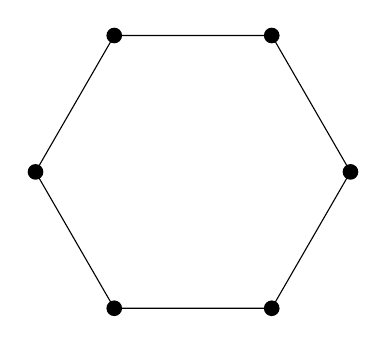
\begin{tikzpicture}
        % Defining the vertices of the cycle
        \foreach \x in {0,60,...,300} {
                \node[circle, fill=black, inner sep=2pt] at (\x:2) {};
            }
        % Drawing the edges of the cycle
        \draw (0:2) -- (60:2) -- (120:2) -- (180:2) -- (240:2) -- (300:2) -- cycle;
    \end{tikzpicture}

    \pause
    Primer za \(n\)-cikel.
    \[c(C_n) = \frac{2}{\lfloor \frac n2\rfloor}\]
\end{frame}
\begin{frame}{Primeri - Cheegerjeva konstanta}
    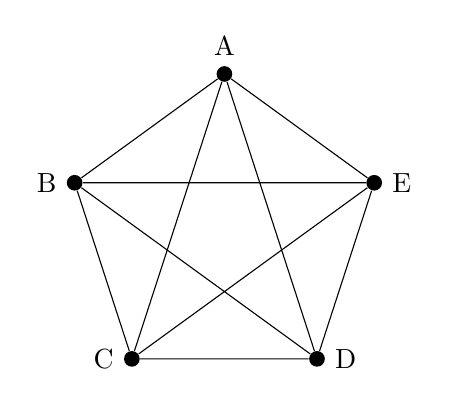
\begin{tikzpicture}
        \node[circle, fill=black, inner sep=2pt, label=above:A] (A) at (90:2) {};
        \node[circle, fill=black, inner sep=2pt, label=left:B] (B) at (162:2) {};
        \node[circle, fill=black, inner sep=2pt, label=left:C] (C) at (234:2) {};
        \node[circle, fill=black, inner sep=2pt, label=right:D] (D) at (306:2) {};
        \node[circle, fill=black, inner sep=2pt, label=right:E] (E) at (18:2) {};
        \draw (A) -- (B) -- (C) -- (D) -- (E) -- (A);
        \draw (A) -- (C) -- (E) -- (B) -- (D) -- (A);
    \end{tikzpicture}
    \pause
    Primer za \(K_n\).
    \[c(K_n) = \lceil \frac n2\rceil\]
\end{frame}
% END CHEEGER
% BEGIN SPECTRAL GAP
\begin{frame}{Spektralna luknja}
    Obstaja soroden pojem Cheegerjeve konstante - spektralna luknja.

    \(\lambda_i\) lastne vrednosti sosednostne matrike grafov.
    \[
        \lambda_1 \geq \lambda_2 \geq \ldots \geq \lambda_n
    \]

    \[
        s(G) = \lambda_1 - \lambda_2
    \]
\end{frame}
\begin{frame}{Lastne vrednosti grafov - primeri}
    \begin{itemize}
        \item \(K_n\) - \(n-1, -1, \ldots, -1\)
        \item \(K_{d,d}\) - \(d,\)
    \end{itemize}
\end{frame}
\begin{frame}{Spektralna luknja - primeri}
    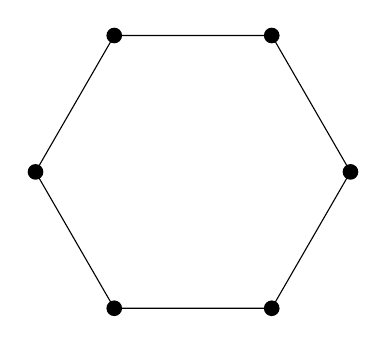
\begin{tikzpicture}
        % Defining the vertices of the cycle
        \foreach \x in {0,60,...,300} {
                \node[circle, fill=black, inner sep=2pt] at (\x:2) {};
            }
        % Drawing the edges of the cycle
        \draw (0:2) -- (60:2) -- (120:2) -- (180:2) -- (240:2) -- (300:2) -- cycle;
    \end{tikzpicture}

    \pause
    Primer za \(n\)-cikel.
    \[c(G) = \frac{2}{\lfloor \frac n2\rfloor}\]
\end{frame}
% END SPECTRAL GAP
\begin{frame}{Caylejevi grafi \(\mathbb Z_4\)}
    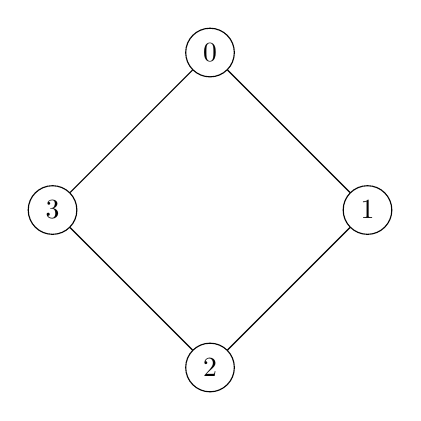
\begin{tikzpicture}
        % Define the style for the nodes
        \tikzset{every node/.style={draw,circle}}

        % Nodes
        \node (1) at (0,2) {0};
        \node (2) at (2,0) {1};
        \node (3) at (0,-2) {2};
        \node (4) at (-2,0) {3};

        % Edges
        \draw (1) -- (2);
        \draw (2) -- (3);
        \draw (3) -- (4);
        \draw (4) -- (1);
    \end{tikzpicture}
\end{frame}

\end{document}
